\section{Skip List implementation}
\subsection{Introduction}
The purpose of this chapter is to report the tests that have been done to find the best value of \underline{height} in a Skip List.
Skip List is a probabilistic data structure that allows searching, insertion and deleting operation with time complexity of $O(log n)$.

\subsection{Testing methodology\footnote{all test are done on a Lenovo Thinkpad x390 yoga with an Intel Core i7-8565U CPU and 16GB of RAM, with Arch Linux installed as only OS}}
I wrote a python script that runs the program with different values of \underline{height} and saves the output in a file, the range of tested level is between 6 and 50
\newline
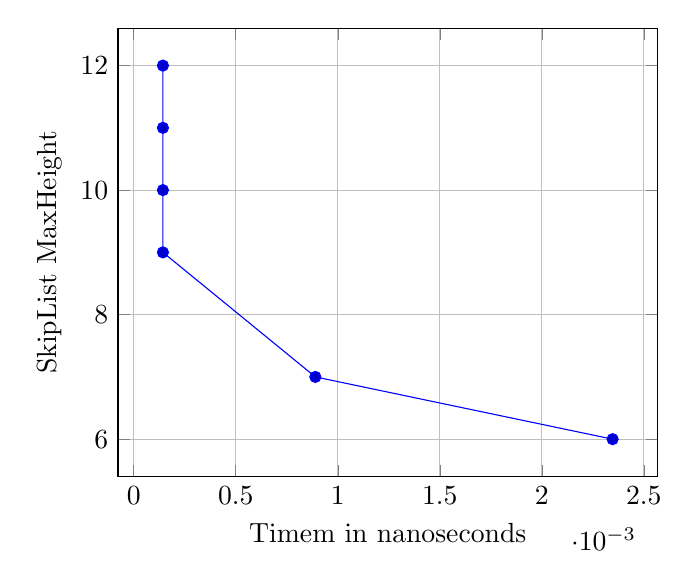
\begin{tikzpicture}
  \begin{axis}[
    xlabel={Timem in nanoseconds},
    ylabel={SkipList MaxHeight},
    grid=major,
    legend pos=north west,
  ]

  % Add your data points here
  % The 'nan' values indicate that the algorithm did not terminate for those max_height values
  \addplot+[
    error bars/.cd,
    y dir=both,
    y explicit,
    error bar style={line width=1pt},
  ] coordinates {
    (nan,1) 
    (nan,2)
    (nan,3)
    (nan,4)
    (nan,5)% Add 'nan' for values where the algorithm did not finish
    (0.002347,6)
    (0.000890,7)
    (0.000143,9)
    (0.000143,10)
    (0.000143,11)
    (0.000143,12)
    % Add more data points and 'nan' as needed
  };


  \end{axis}
\end{tikzpicture}
\newline
Range from 1 to 5 is omitted because the algorithm did not terminate for those values